%%%%%%%%%%%%%%%%%%%%%%%%%%%%%%%%%%%%%%%%%%%%%%%%%%%%%%%%%%%%%%%
%% Copyright 2009 Ivan Griffin
%  Copyright 2015 Paul Danese
% Adapted from Ivan Griffin's work (http://www.texample.net/tikz/examples/author/ivan-griffin/)
% I have no idea how copyright works. Hopefully, I'm not breaking any rules / laws or stepping on any toes. 
% If I am breaking rules / laws / toes, it was unintentional.
% This work may be distributed and/or modified under the
% conditions of the LaTeX Project Public License, either version 1.3
% of this license or (at your option) any later version.
% The latest version of this license is in
%   http://www.latex-project.org/lppl.txt
% and version 1.3 or later is part of all distributions of LaTeX
% version 2005/12/01 or later.
%
% This work has the LPPL maintenance status `maintained'.
% 
% The Current Maintainer of this work is Paul Danese
%
% This work consists of the files periodic_table.tex

%Description
%Created 2009-12-08 by Ivan Griffin.  Last updated: 2010-01-11
% Modified 2015-10-24 by Paul Danese
%Thanks to Jerome. Thanks to Ivan.
%-------------------------------------------------------------

\documentclass[9pt]{article}
\usepackage[margin=0.3in]{geometry}
\usepackage{tikz}
\usepackage{hyperref}
\usetikzlibrary{shapes}
% wanted to use the standard latex serif font, which I like.
% also wanted to avoid excessive coloring of different element groups (e.g., noble gases, alkalai metals, etc.)



\begin{document}
\pagenumbering{gobble} % suppress page numbering here
\newcommand{\NaturalElementTextFormat}[4]
{
  \begin{minipage}{2.33cm}
    \centering
      \textbf{#1}
      \\[0.1cm]
      {\Huge \textbf{{#3}}}
      \linebreak
       {#4}
      \linebreak
      {\small {#2}} 
  \end{minipage}
}

\newcommand{\KeyTextFormat}[4]
{
	\begin{minipage}{2.3cm}
		\centering
		\textbf{#1}
		\\[0.1cm]
		{\Large \textbf{{#3}}}
		\linebreak
		{#4}
		\linebreak
		{\small {#2}} 
	\end{minipage}
}


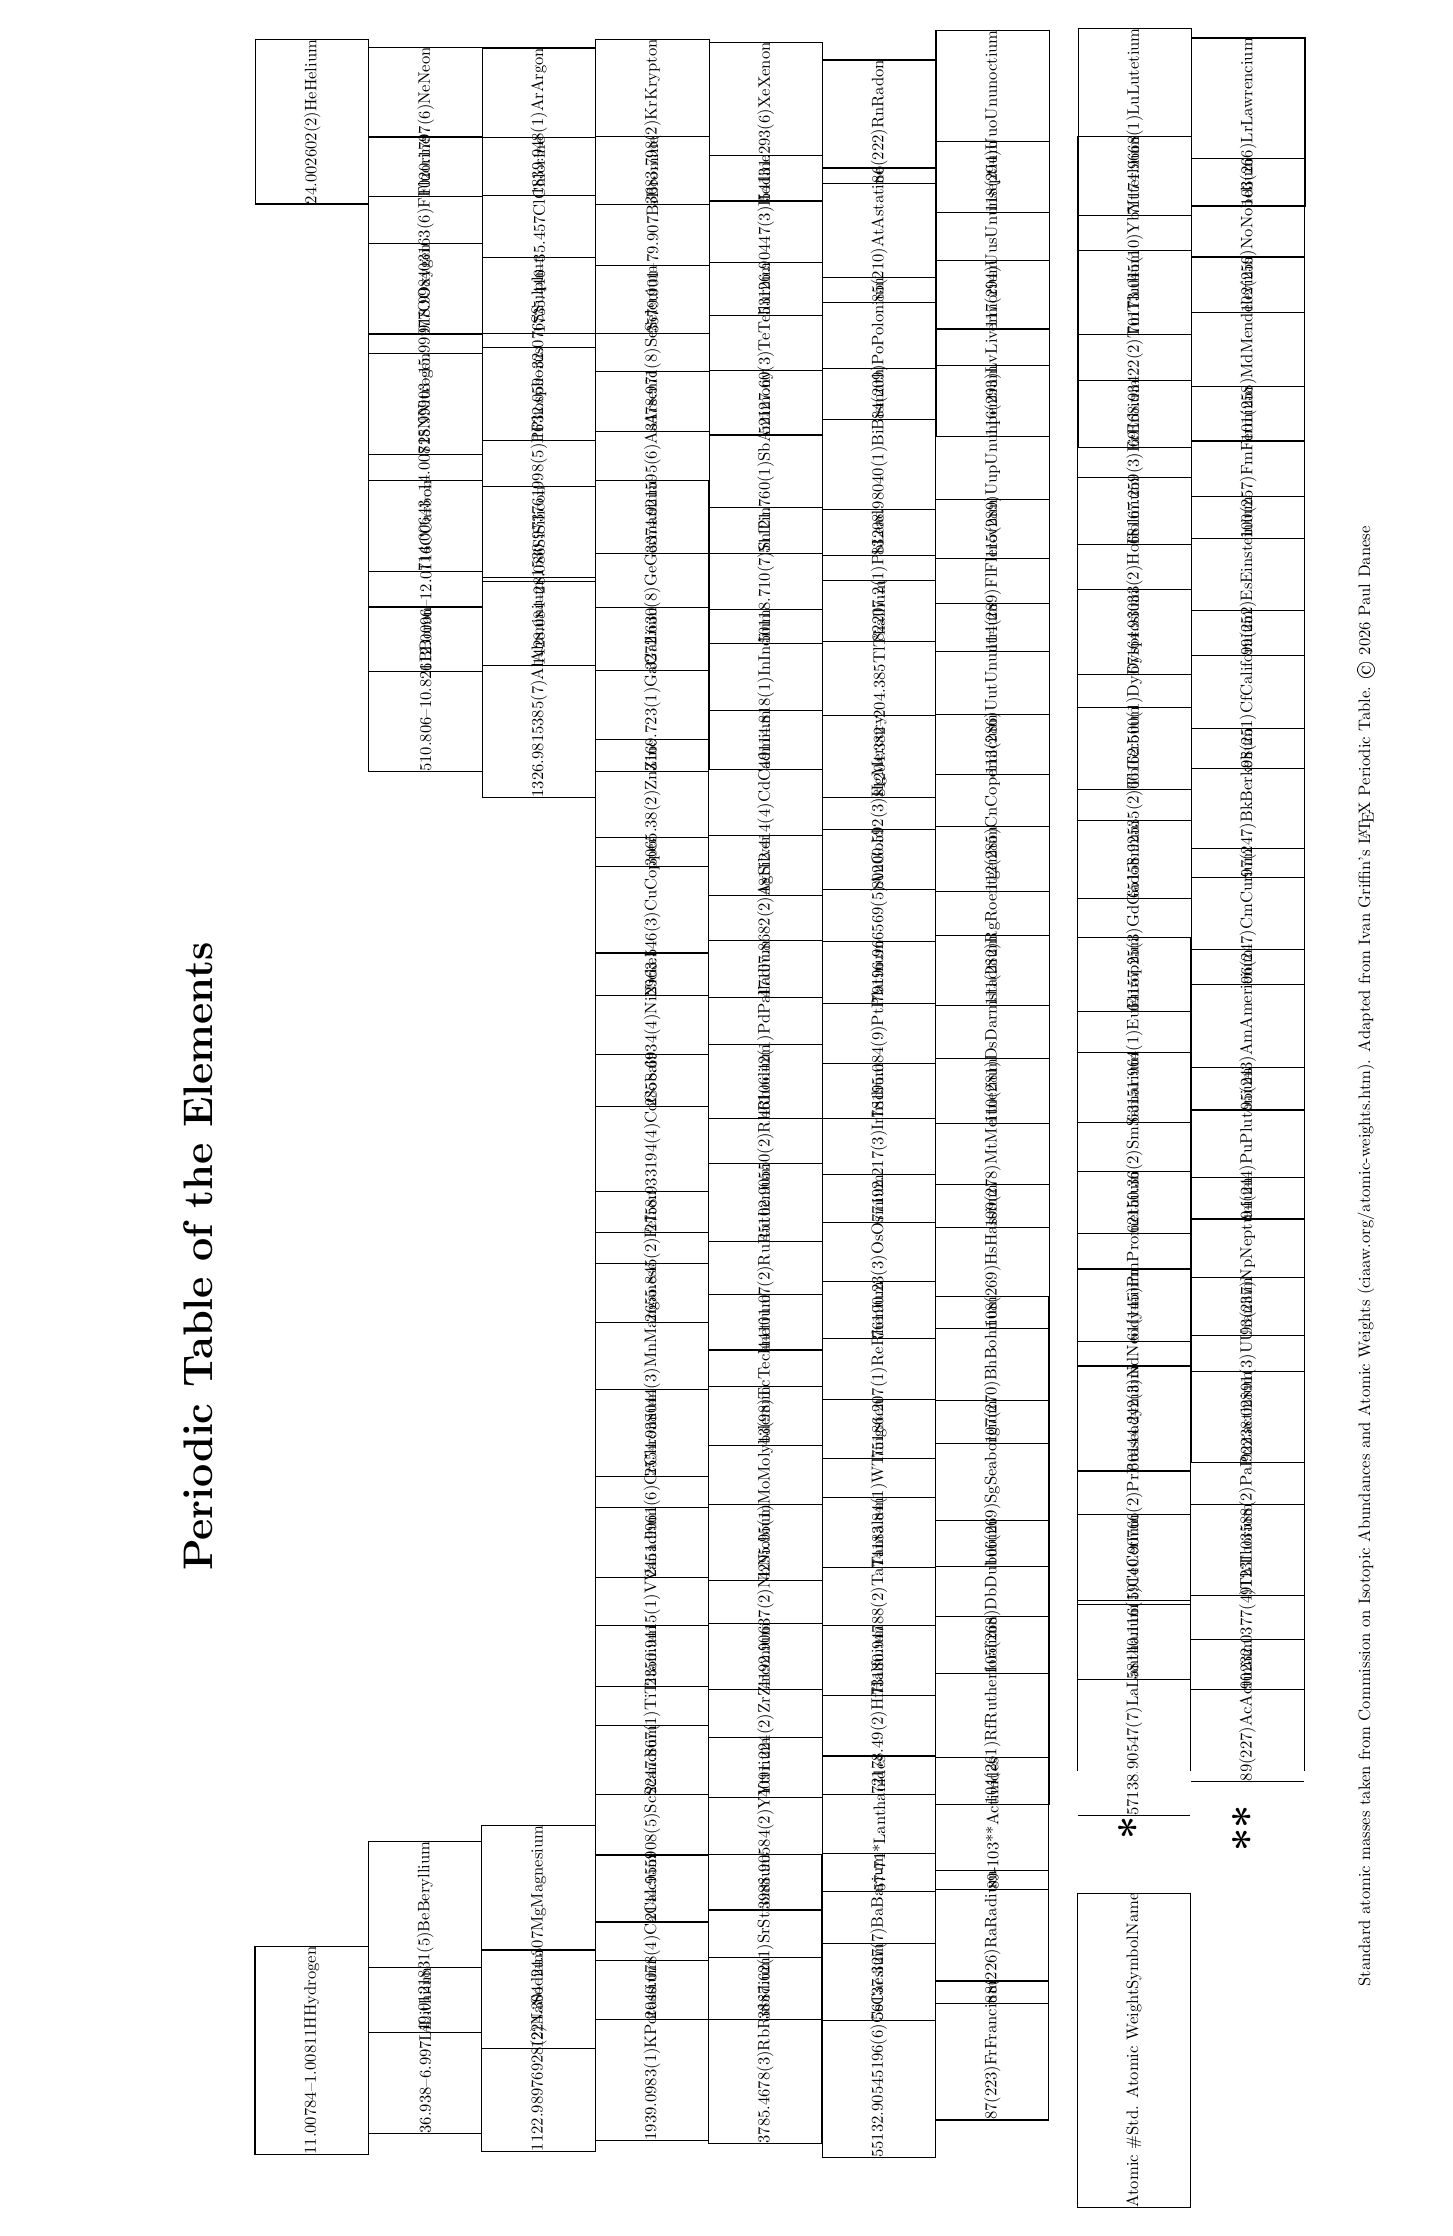
\begin{tikzpicture}[scale=0.6, transform shape, rotate=90]

\tikzstyle{Element} = [draw=black, minimum width=2.4cm, minimum height=2.4cm, node distance=2.4cm, inner sep=0pt]
\tikzstyle{Offsetter} = [draw=white, minimum width=2.4cm, minimum height=2.4cm, node distance=2.4cm, inner sep=0pt]
\tikzstyle{TitleLabel} = [font={\Huge\bfseries}]
\tikzstyle{DetailsLabel} = [minimum height = 2.5cm, node distance = 2.5cm, inner sep=0pt]

%% Group 1 - IA
  \node[name=Blank1, Offsetter] {}; % this is just an invisible box that shoves the entire table downward to make it more centered
  \node[name=Blank2, below of=Blank1, Offsetter] {}; % see comment on invisible box above.
  \node[name=H,below of=Blank2, Element] {\NaturalElementTextFormat{1}{1.00784--1.00811}{H}{Hydrogen}};
  \node[name=Li, below of=H, Element] {\NaturalElementTextFormat{3}{6.938--6.997}{Li}{Lithium}};
  \node[name=Na, below of=Li, Element] {\NaturalElementTextFormat{11}{22.98976928(2)}{Na}{Sodium}};
  \node[name=K, below of=Na, Element] {\NaturalElementTextFormat{19}{39.0983(1)}{K}{Potassium}};
  \node[name=Rb, below of=K, Element] {\NaturalElementTextFormat{37}{85.4678(3)}{Rb}{Rubidium}};
  \node[name=Cs, below of=Rb, Element] {\NaturalElementTextFormat{55}{132.90545196(6)}{Cs}{Caesium}};
  \node[name=Fr, below of=Cs, Element] {\NaturalElementTextFormat{87}{(223)}{Fr}{Francium}};

%% Group 2 - IIA
  \node[name=Be, right of=Li, Element] {\NaturalElementTextFormat{4}{9.0121831(5)}{Be}{Beryllium}};
  \node[name=Mg, below of=Be, Element] {\NaturalElementTextFormat{12}{24.304--24.307}{Mg}{Magnesium}};
  \node[name=Ca, below of=Mg, Element] {\NaturalElementTextFormat{20}{40.078(4)}{Ca}{Calcium}};
  \node[name=Sr, below of=Ca, Element] {\NaturalElementTextFormat{38}{87.62(1)}{Sr}{Strontium}};
  \node[name=Ba, below of=Sr, Element] {\NaturalElementTextFormat{56}{137.327(7)}{Ba}{Barium}};
  \node[name=Ra, below of=Ba, Element] {\NaturalElementTextFormat{88}{(226)}{Ra}{Radium}};

%% Group 3 - IIIB
  \node[name=Sc, right of=Ca, Element] {\NaturalElementTextFormat{21}{44.955908(5)}{Sc}{Scandium}};
  \node[name=Y, below of=Sc, Element] {\NaturalElementTextFormat{39}{88.90584(2)}{Y}{Yttrium}};
  \node[name=LaLu, below of=Y, Element] {\NaturalElementTextFormat{57-71}{}{*}{Lanthanides}};
d  \node[name=AcLr, below of=LaLu, Element] {\NaturalElementTextFormat{89-103}{}{**}{Actinides}};

%% Group 4 - IVB
  \node[name=Ti, right of=Sc, Element] {\NaturalElementTextFormat{22}{47.867(1)}{Ti}{Titanium}};
  \node[name=Zr, below of=Ti, Element] {\NaturalElementTextFormat{40}{91.224(2)}{Zr}{Zirconium}};
  \node[name=Hf, below of=Zr, Element] {\NaturalElementTextFormat{72}{178.49(2)}{Hf}{Halfnium}};
  \node[name=Rf, below of=Hf, Element] {\NaturalElementTextFormat{104}{(261)}{Rf}{Rutherfordium}};

%% Group 5 - VB
  \node[name=V, right of=Ti, Element] {\NaturalElementTextFormat{23}{50.9415(1)}{V}{Vanadium}};
  \node[name=Nb, below of=V, Element] {\NaturalElementTextFormat{41}{92.90637(2)}{Nb}{Niobium}};
  \node[name=Ta, below of=Nb, Element] {\NaturalElementTextFormat{73}{180.94788(2)}{Ta}{Tantalum}};
  \node[name=Db, below of=Ta, Element] {\NaturalElementTextFormat{105}{(268)}{Db}{Dubnium}};

%% Group 6 - VIB
  \node[name=Cr, right of=V, Element] {\NaturalElementTextFormat{24}{51.9961(6)}{Cr}{Chromium}};
  \node[name=Mo, below of=Cr, Element] {\NaturalElementTextFormat{42}{95.95(1)}{Mo}{Molybdenum}};
  \node[name=W, below of=Mo, Element] {\NaturalElementTextFormat{74}{183.84(1)}{W}{Tungsten}};
  \node[name=Sg, below of=W, Element] {\NaturalElementTextFormat{106}{(269)}{Sg}{Seaborgium}};

%% Group 7 - VIIB
  \node[name=Mn, right of=Cr, Element] {\NaturalElementTextFormat{25}{54.938044(3)}{Mn}{Manganese}};
  \node[name=Tc, below of=Mn, Element] {\NaturalElementTextFormat{43}{(98)}{Tc}{Technetium}};
  \node[name=Re, below of=Tc, Element] {\NaturalElementTextFormat{75}{186.207(1)}{Re}{Rhenium}};
  \node[name=Bh, below of=Re, Element] {\NaturalElementTextFormat{107}{(270)}{Bh}{Bohrium}};

%% Group 8 - VIIIB
  \node[name=Fe, right of=Mn, Element] {\NaturalElementTextFormat{26}{55.845(2)}{Fe}{Iron}};
  \node[name=Ru, below of=Fe, Element] {\NaturalElementTextFormat{44}{101.07(2)}{Ru}{Ruthenium}};
  \node[name=Os, below of=Ru, Element] {\NaturalElementTextFormat{76}{190.23(3)}{Os}{Osmium}};
  \node[name=Hs, below of=Os, Element] {\NaturalElementTextFormat{108}{(269)}{Hs}{Hassium}};

%% Group 9 - VIIIB
  \node[name=Co, right of=Fe, Element] {\NaturalElementTextFormat{27}{58.933194(4)}{Co}{Cobalt}};
  \node[name=Rh, below of=Co, Element] {\NaturalElementTextFormat{45}{102.90550(2)}{Rh}{Rhodium}};
  \node[name=Ir, below of=Rh, Element] {\NaturalElementTextFormat{77}{192.217(3)}{Ir}{Iridium}};
  \node[name=Mt, below of=Ir, Element] {\NaturalElementTextFormat{109}{(278)}{Mt}{Meitnerium}};

%% Group 10 - VIIIB
  \node[name=Ni, right of=Co, Element] {\NaturalElementTextFormat{28}{58.6934(4)}{Ni}{Nickel}};
  \node[name=Pd, below of=Ni, Element] {\NaturalElementTextFormat{46}{106.42(1)}{Pd}{Palladium}};
  \node[name=Pt, below of=Pd, Element] {\NaturalElementTextFormat{78}{195.084(9)}{Pt}{Platinum}};
  \node[name=Ds, below of=Pt, Element] {\NaturalElementTextFormat{110}{(281)}{Ds}{Darmstadtium}};

%% Group 11 - IB
  \node[name=Cu, right of=Ni, Element] {\NaturalElementTextFormat{29}{63.546(3)}{Cu}{Copper}};
  \node[name=Ag, below of=Cu, Element] {\NaturalElementTextFormat{47}{107.8682(2)}{Ag}{Silver}};
  \node[name=Au, below of=Ag, Element] {\NaturalElementTextFormat{79}{196.966569(5)}{Au}{Gold}};
  \node[name=Rg, below of=Au, Element] {\NaturalElementTextFormat{111}{(282)}{Rg}{Roentgenium}};

%% Group 12 - IIB
  \node[name=Zn, right of=Cu, Element] {\NaturalElementTextFormat{30}{65.38(2)}{Zn}{Zinc}};
  \node[name=Cd, below of=Zn, Element] {\NaturalElementTextFormat{48}{112.414(4)}{Cd}{Cadmium}};
  \node[name=Hg, below of=Cd, Element] {\NaturalElementTextFormat{80}{200.592(3)}{Hg}{Mercury}};
  \node[name=Uub, below of=Hg, Element] {\NaturalElementTextFormat{112}{(285)}{Cn}{Copernicium}};

%% Group 13 - IIIA
  \node[name=Ga, right of=Zn, Element] {\NaturalElementTextFormat{31}{69.723(1)}{Ga}{Gallium}};
  \node[name=Al, above of=Ga, Element] {\NaturalElementTextFormat{13}{26.9815385(7)}{Al}{Aluminium}};
  \node[name=B, above of=Al, Element] {\NaturalElementTextFormat{5}{10.806--10.821}{B}{Boron}};
  \node[name=In, below of=Ga, Element] {\NaturalElementTextFormat{49}{114.818(1)}{In}{Indium}};
  \node[name=Tl, below of=In, Element] {\NaturalElementTextFormat{81}{204.382--204.385}{Tl}{Thallium}};
  \node[name=Uut, below of=Tl, Element] {\NaturalElementTextFormat{113}{(286)}{Uut}{Ununtrium}};

%% Group 14 - IVA
  \node[name=C, right of=B, Element] {\NaturalElementTextFormat{6}{12.0096--12.0116}{C}{Carbon}};
  \node[name=Si, below of=C, Element] {\NaturalElementTextFormat{14}{28.084--28.086}{Si}{Silicon}};
  \node[name=Ge, below of=Si, Element] {\NaturalElementTextFormat{32}{72.630(8)}{Ge}{Germanium}};
  \node[name=Sn, below of=Ge, Element] {\NaturalElementTextFormat{50}{118.710(7)}{Sn}{Tin}};
  \node[name=Pb, below of=Sn, Element] {\NaturalElementTextFormat{82}{207.2(1)}{Pb}{Lead}};
  \node[name=Uuq, below of=Pb, Element] {\NaturalElementTextFormat{114}{(289)}{Fl}{Flerovium}};

%% Group 15 - VA
  \node[name=N, right of=C, Element] {\NaturalElementTextFormat{7}{14.00643--14.00728}{N}{Nitrogen}};
  \node[name=P, below of=N, Element] {\NaturalElementTextFormat{15}{30.973761998(5)}{P}{Phosphorus}};
  \node[name=As, below of=P, Element] {\NaturalElementTextFormat{33}{74.921595(6)}{As}{Arsenic}};
  \node[name=Sb, below of=As, Element] {\NaturalElementTextFormat{51}{121.760(1)}{Sb}{Antimony}};
  \node[name=Bi, below of=Sb, Element] {\NaturalElementTextFormat{83}{208.98040(1)}{Bi}{Bismuth}};
  \node[name=Uup, below of=Bi, Element] {\NaturalElementTextFormat{115}{(289)}{Uup}{Ununpentium}};

%% Group 16 - VIA
  \node[name=O, right of=N, Element] {\NaturalElementTextFormat{8}{15.99903--15.99977}{O}{Oxygen}};
  \node[name=S, below of=O, Element] {\NaturalElementTextFormat{16}{32.059--32.076}{S}{Sulphur}};
  \node[name=Se, below of=S, Element] {\NaturalElementTextFormat{34}{78.971(8)}{Se}{Selenium}};
  \node[name=Te, below of=Se, Element] {\NaturalElementTextFormat{52}{127.60(3)}{Te}{Tellurium}};
  \node[name=Po, below of=Te, Element] {\NaturalElementTextFormat{84}{(209)}{Po}{Polonium}};
  \node[name=Uuh, below of=Po, Element] {\NaturalElementTextFormat{116}{(293)}{Lv}{Livermorium}};

%% Group 17 - VIIA
  \node[name=F, right of=O, Element] {\NaturalElementTextFormat{9}{18.998403163(6)}{F}{Fluorine}};
  \node[name=Cl, below of=F, Element] {\NaturalElementTextFormat{17}{35.446--35.457}{Cl}{Chlorine}};
  \node[name=Br, below of=Cl, Element] {\NaturalElementTextFormat{35}{79.901--79.907}{Br}{Bromine}};
  \node[name=I, below of=Br, Element] {\NaturalElementTextFormat{53}{126.90447(3)}{I}{Iodine}};
  \node[name=At, below of=I, Element] {\NaturalElementTextFormat{85}{(210)}{At}{Astatine}};
  \node[name=Uus, below of=At, Element] {\NaturalElementTextFormat{117}{(294)}{Uus}{Ununseptium}}; 

%% Group 18 - VIIIA
  \node[name=Ne, right of=F, Element] {\NaturalElementTextFormat{10}{20.1797(6)}{Ne}{Neon}};
  \node[name=He, above of=Ne, Element] {\NaturalElementTextFormat{2}{4.002602(2)}{He}{Helium}};
  \node[name=Ar, below of=Ne, Element] {\NaturalElementTextFormat{18}{39.948(1)}{Ar}{Argon}};
  \node[name=Kr, below of=Ar, Element] {\NaturalElementTextFormat{36}{83.798(2)}{Kr}{Krypton}};
  \node[name=Xe, below of=Kr, Element] {\NaturalElementTextFormat{54}{131.293(6)}{Xe}{Xenon}};
  \node[name=Rn, below of=Xe, Element] {\NaturalElementTextFormat{86}{(222)}{Rn}{Radon}};
  \node[name=Uuo, below of=Rn, Element] {\NaturalElementTextFormat{118}{(294)}{Uuo}{Ununoctium}}; 


%% Lanthanide
  \node[name=La, below of=Rf, Element, yshift=-0.6cm] {\NaturalElementTextFormat{57}{138.90547(7)}{La}{Lanthanum}};
  \node[name=Ce, right of=La, Element] {\NaturalElementTextFormat{58}{140.116(1)}{Ce}{Cerium}};
  \node[name=Pr, right of=Ce, Element] {\NaturalElementTextFormat{59}{140.90766(2)}{Pr}{Praseodymium}};
  \node[name=Nd, right of=Pr, Element] {\NaturalElementTextFormat{60}{144.242(3)}{Nd}{Neodymium}};
  \node[name=Pm, right of=Nd, Element] {\NaturalElementTextFormat{61}{(145)}{Pm}{Promethium}};
  \node[name=Sm, right of=Pm, Element] {\NaturalElementTextFormat{62}{150.36(2)}{Sm}{Samarium}};
  \node[name=Eu, right of=Sm, Element] {\NaturalElementTextFormat{63}{151.964(1)}{Eu}{Europium}};
  \node[name=Gd, right of=Eu, Element] {\NaturalElementTextFormat{64}{157.25(3)}{Gd}{Gadolinium}};
  \node[name=Tb, right of=Gd, Element] {\NaturalElementTextFormat{65}{158.92535(2)}{Tb}{Terbium}};
  \node[name=Dy, right of=Tb, Element] {\NaturalElementTextFormat{66}{162.500(1)}{Dy}{Dysprosium}};
  \node[name=Ho, right of=Dy, Element] {\NaturalElementTextFormat{67}{164.93033(2)}{Ho}{Holmium}};
  \node[name=Er, right of=Ho, Element] {\NaturalElementTextFormat{68}{167.259(3)}{Er}{Erbium}};
  \node[name=Tm, right of=Er, Element] {\NaturalElementTextFormat{69}{168.93422(2)}{Tm}{Thulium}};
  \node[name=Yb, right of=Tm, Element] {\NaturalElementTextFormat{70}{173.045(10)}{Yb}{Ytterbium}};
  \node[name=Lu, right of=Yb, Element] {\NaturalElementTextFormat{71}{174.9668(1)}{Lu}{Lutetium}};

%% Actinide
  \node[name=Ac, below of=La, Element] {\NaturalElementTextFormat{89}{(227)}{Ac}{Actinium}};
  \node[name=Th, right of=Ac, Element] {\NaturalElementTextFormat{90}{232.0377(4)}{Th}{Thorium}};
  \node[name=Pa, right of=Th, Element] {\NaturalElementTextFormat{91}{231.03588(2)}{Pa}{Protactinium}};
  \node[name=U, right of=Pa, Element] {\NaturalElementTextFormat{92}{238.02891(3)}{U}{Uranium}};
  \node[name=Np, right of=U, Element] {\NaturalElementTextFormat{93}{(237)}{Np}{Neptunium}};
  \node[name=Pu, right of=Np, Element] {\NaturalElementTextFormat{94}{(244)}{Pu}{Plutonium}};
  \node[name=Am, right of=Pu, Element] {\NaturalElementTextFormat{95}{(243)}{Am}{Americium}};
  \node[name=Cm, right of=Am, Element] {\NaturalElementTextFormat{96}{(247)}{Cm}{Curium}};
  \node[name=Bk, right of=Cm, Element] {\NaturalElementTextFormat{97}{(247)}{Bk}{Berkelium}};
  \node[name=Cf, right of=Bk, Element] {\NaturalElementTextFormat{98}{(251)}{Cf}{Californium}};
  \node[name=Es, right of=Cf, Element] {\NaturalElementTextFormat{99}{(252)}{Es}{Einsteinium}};
  \node[name=Fm, right of=Es, Element] {\NaturalElementTextFormat{100}{(257)}{Fm}{Fermium}};
  \node[name=Md, right of=Fm, Element] {\NaturalElementTextFormat{101}{(258)}{Md}{Mendelevium}};
  \node[name=No, right of=Md, Element] {\NaturalElementTextFormat{102}{(259)}{No}{Nobelium}};
  \node[name=Lr, right of=No, Element] {\NaturalElementTextFormat{103}{(266)}{Lr}{Lawrencium}};
  \node[name=Star, left of=La, Offsetter, xshift=-0.1cm] {{\textbf{\Huge *}}};
  \node[name=DoubleStar, below of=Star, Offsetter] {{\textbf{\Huge **}}};

  \node[name=Key, below of=Fr, Element, yshift=-0.6cm] {\KeyTextFormat{Atomic \#}{Std. Atomic Weight}{Symbol}{Name}};

\node at (Blank2.west -| Fe.north) [name=diagramTitle, TitleLabel]
{Periodic Table of the Elements};

\node[below of=Np, name=details, DetailsLabel]{Standard atomic masses taken from Commission on Isotopic Abundances and Atomic Weights (ciaaw.org/atomic-weights.htm). Adapted from Ivan Griffin's \LaTeX\space Periodic Table. \textcopyright\space \the\year\space Paul Danese};
\end{tikzpicture}
\end{document}